% !TeX root = main.tex
% !TeX spellcheck = en-US
% !TeX encoding = utf8


\chapter{Experimental Design and Tests}
\label{chap:experiment}

\section{Choice of Problem Instances}
\label{chap:problem-choice}

This thesis builds on the foundation of the \glsfirst{hsppbo} work of \citet{kupfer2021hierarchical}. Therefore, the problem category was chosen analogously to the symmetric \glsfirst{tsp}. In this way, we can refer to previous work, while also generalizing many different, relevant problems (see \cref{chap:tsp}). 
The \gls{tsp} instance test cases were taken from the popular \textit{TSPLIB} benchmarking suite \cite{reinelt1991tsplib}, since they have been tried and tested in many publications and also have the advantage that the optimal solution is known for each of the problems, which enables further comparison with other metaheuristics. Besides the standard 2D Euclidean weights, there are also instances of geographic distance problems or distance matrices. The thesis focuses on 2D Euclidean instances for simplicity, but the software itself can handle most types of TSP edge weights (see \cref{chap:tsp-module}).

The thesis also aims at solving the \glsfirst{dtsp}. However, the dynamic part is implemented by the \texttt{problem} module itself, and is not a standard part of the \textit{TSPLIB} library. All \textit{TSPLIB} instances have a different number of cities $n$ (called dimension in the following), and often certain characteristics by which the cities are placed in their space, sometimes described in the \textit{TSPLIB} file (under \texttt{COMMENT}). An example of such a file is shown in \cref{lst:tsp-file}. To quantify these cases, several statistical values have been calculated for the corresponding distance matrices. These provide a way to select a meaningful, disjoint subset of problem instances without using too many, since the computational cost of running the larger instances can be quite significant.

\begin{Listing}
	\begin{minted}{text}
		
NAME : bier127
COMMENT : 127 Biergaerten in Augsburg (Juenger/Reinelt)
TYPE : TSP
DIMENSION : 127
EDGE_WEIGHT_TYPE : EUC_2D
NODE_COORD_SECTION
1   9860  14152
2   9396  14616
[...]
127   3248  14152
EOF
	\end{minted}
	\caption{The \textit{TSPLIB} file for the \texttt{bier127} problem instance (node list shortened).}
	\label{lst:tsp-file}
\end{Listing}


The selection of problem instances was influenced by two metrics: dimension $n$ and city placement characteristics. Since this implementation of the \gls{hsppbo} algorithm scales linearly with $n$, and the \glsfirst{hpo} process runs the algorithm multiple times (\texttt{n\_calls}), with the optimization also being repeated multiple times ($r_\text{opt}$) for each dynamic configuration and problem instance $\mathcal{P}$, the maximum dimension used is 450 to keep the computation time within a reasonable limit. The lower bound for the dimension $n$ is 50, since smaller instances make it difficult to detect any placement characteristics. This results in a dimension bounded by the interval $[50,450]$, which is then roughly divided into smaller instances (50-250 cities) and larger instances (250-450).

With the dimension partitioned, we are left with the statistical measures to analyze the placement characteristic. These measures have been chosen for their expressiveness in graph and distribution problems. Furthermore, it should be possible to calculate them as fast as possible. In order to justify the final choice of \gls{tsp} instances, various literature was searched for similar procedures.
Under the assumption that similarly structured \gls{tsp} instances share common parameter values for their metaheuristic solvers, the following problem classification aims to be very thorough, so that all parameters obtained for the smaller instances can later be used for the larger instances as well.

\subsection{Statistical Measures for Analysis}
\label{chap:prob-stat-meas}

The city placement characteristic was determined using the following statistical values, which was computed for each \textit{TSPLIB} instance over the corresponding distance matrix $D$ using the \textit{NumPy} package \cite{harris2020array}:

\begin{itemize}
	\item The mean $\mu$, median $\tilde{d}$ and standard deviation $\sigma$
	\item The coefficient of variation $c_\text{v}$
	\item The coefficient of quartile variation (CQV)
	\item The regularity index $R$
	\item The first eigenvalue $\lambda_1$
	\item The \enquote{eigen gap} $\Delta\lambda_{1,2}$, i.e. the gap between the first two eigenvalues
\end{itemize}

The mean, median, and standard deviation are common choices for analyzing data sets. These three values  already make it possible to give a first impression of how evenly the city nodes are distributed in Euclidean space. For example, if the mean distance between nodes differs greatly from the median with a high standard deviation, we can assume that the instance is somewhat unevenly distributed. However, since these values are absolute and therefore dependent on the problem and its distance scaling, they cannot be used for comparison across all instances.
Since we want to identify distributions and clusters within the \gls{tsp} instances, measures of statistical dispersion were preferred for further calculations. These provide insight into how compressed or stretched out a data set is. Furthermore, only dimensionless metrics were considered.

One possible measure of dispersion is the coefficient of variation, which improves on the standard deviation by effectively normalizing it by division with the mean: $c_\text{v} = \frac{\sigma}{\mu}$. This results in a relative value that can be used comparatively. However, the coefficient of variation tends to overexpose outliers, which may be undesirable when classifying highly clustered instances.
Another measure is the \gls{cqv}, which is a robust version of the coefficient of variation and therefore less sensitive to outliers \cite{bonett2006confidence}. It is defined as $CQV = \frac{Q_3 - Q_1}{Q_3 + Q_1}$, where $Q_1$ and $Q_3$ are the first and third quartiles of the distance matrices distribution.

The regularity index $R$ is a metric that was developed especially for the quantification of spatial distributions by \citet{clark1954distance}. It is defined as the ratio between the median distance between each nearest neighbor $r_A$ and the median distance between nearest neighbors under the assumption of a perfect random distribution $r_E$, specified by a density $\rho$, so that $R = r_A / r_E$.
Thus, a value of $R = 1$ would indicate a completely random distribution, while $R = 0$ would suggest that all nodes are located at the same position.
In order to compute this measure effectively, some considerations had to be made.
The numerator $r_A$ is easily calculated by using the minimum function over all possible distances for each node \cite{dry2012clustering}: 
\begin{equation}
	r_A = \frac{1}{n} \sum_{i \neq j}^{n} \min(d_{ij})
\end{equation}
In this case, however, the distance under random distribution depends on the area $A$ and the number of nodes $n$, with a point density of $\delta = n/A$. The formula for $r_E$ is described by a Poisson process for complete spatial randomness. By making some adjustments to incorporate a sense of absolute distance and taking the expectation of the resulting probability distribution, we get the following formula \cite{dry2012clustering}:
\begin{equation}
	r_E = \frac{1}{2} \sqrt{\frac{A}{n}}
\end{equation}
The area $A$ covered by the nodes, i.e. the convex hull of the graph, was obtained using the \textit{SciPy} library \cite{2020SciPy-NMeth}, which provides algorithms for scientific computing in \textit{Python}.
Although not originally applied to the \gls{tsp}, the works of \citet{dry2012clustering, cricsan2021randomness} give an insight into the suitability of the regularity index for this problem category, concluding that it is highly significant, even if not perfect. Finally, in an application of the research around spectral analysis of graph problems and the \gls{tsp}, the first two (largest) eigenvalues were computed over the distance matrix $D$. While the first eigenvalue can be related to average length of the Hamilton cycle in a \gls{tsp} instance \cite{cvetkovic2018traveling}, the \enquote{gap} between the first two eigenvalues could be used as a measure of connectivity \cite{lovasz20071}.

To have a larger sample set, all of these values were calculated for all \textit{TSPLIB} instances with a dimension less than 1000 and a valid edge weight type for the \gls{xfopt} package. This excluded \textit{ATT}, \textit{EXPLICIT}, and \textit{CEIL\_2D} problems, but included \textit{GEO} and \textit{ATT}, which resulted in metadata for 118 problem instances.

\subsection{Classification}
\label{chap:classification}

Using these statistical measures, three different methods were employed to classify these 118 \gls{tsp} instances. Since these statistics, except for the regularity index $R$, do not provide qualitative information about the type of class the instance belongs to, all of the graphs were also visualized using the \textit{NetworkX} package. This made it possible to interpret the resulting problem groups by formulating the similarities suggested by the classification. The exploration and application of each of these methods has yielded mixed results, with one clear winner.

\subsubsection{Method I - Regularity Index}

The first method is to use certain value ranges of the regularity index $R$ to discriminate between structures. As mentioned above, this procedure and the applicable ranges have already been validated for the application to the \gls{tsp} by previous work. To further replicate the results obtained by \citet{dry2012clustering, cricsan2021randomness}, additional \gls{tsp} instances from the University of Bonn's \textit{Tnm} test data set \cite{hougardy2021hard} and a triangle lattice generated using the aforementioned \textit{NetworkX} package were used. The implementation of this thesis was able to successfully reproduce the $R$ values from both papers, i.e., all the same values for the \textit{Tnm} \gls{tsp} and a value of $R = 2$, for a highly regular, uniformly distributed triangle lattice \cite{dry2012clustering}.
With this foundation established, the first method was applied to the selected \gls{tsp} instances using the following groups and their ranges:
\begin{itemize}
	\item Heavy clusters:	$R < 0.3$
	\item Semi-clustered: $0.3 \leq R < 0.8$
	\item Random Distribution: $0.8 \leq R < 1.2$
	\item Semi-regular: $1.2 \leq R < 1.4$
	\item Regular: $1.4 \leq R$
\end{itemize}
This first method generally worked well and was able to classify each problem into a satisfactory group. However, it was heavily influenced by higher dimensions and artificial patterns, such as with \textit{pcb442} or \textit{ts225} (see \cref{fig:pcb442,fig:ts225} for visualizations), where artificial is meant to describe that the placement of the cities is clearly influenced by a pattern. These instances were almost all incorrectly classified as randomly distributed ($R\approx1$). 
This method alone would not be able to reliably and disjunctively classify the instances.

\subsubsection{Method II - Eigenvalues of the Distance Matrix}

The second method, inspired by \citet{lovasz20071}, of using the gap between the first two eigenvalues of the distance matrix $D$ proved to be impractical to implement, since it could not be calculated directly on the distance matrix, and would instead use its Laplacian, which is computationally infeasible, especially for larger instances. The paper also states its theory on a positive semi-definite matrix, which the distance matrices used here are not. However, applying the \gls{tsp}-related approach of \citet{cvetkovic2018traveling} of using only the first eigenvalue as a classifier for Hamiltonian path length yielded interesting results. While most of the resulting eigenvalue groups were very unsatisfactory, there was one group consisting of all the artificially structured \gls{tsp} instances. Therefore, a combination of the two methods was the logical next step.

\subsubsection{Method III - k-means Clustering }

The first two methods already identified the regularity index and the first eigenvalue as expressive metrics for classification. With the \glsfirst{cqv} as an additional robust measure of dispersion, a successful classification should be possible. However, it is not practical to manually apply value ranges to three metrics. Therefore, a cluster analysis was performed using the k-means algorithm. 

The problem description for the k-means algorithm is given for a set of data points $n$ in $\mathbb{R}^d$. Given a variable number of $k$ centers, select the position of each center that minimizes the total squared distance from each point to its nearest center \cite{arthur2006k}. This NP-hard problem was originally solved by \citet{lloyd1982least}, resulting in \enquote{Lloyd's algorithm}, or \enquote{Voronoi iteration}. It randomly places $k$ centers in Euclidean space and assigns each point to its nearest center. It then computes a Voronoi diagram over the $k$ sites, integrates these cells, and moves the center to the centroid of each cell. This process is repeated until a stagnation condition is registered. The algorithm used for our application is called \textit{k-means++} and is based on this foundation. Instead of opting for an exact solution, \citet{arthur2006k} propose an approximate procedure to compute the initial $k$ centers. This way, fewer iterations of the otherwise same algorithm are needed to achieve converging behavior and thus satisfactory clusters. 

\begin{figure}
	\centering
	\includegraphics[width=0.9\textwidth]{clusters_kmeans.png}
	\caption[Visualization of the k-means cluster analysis]{Visualization of the k-means cluster analysis applied to 118 \gls{tsp} instances using $k=5$ clusters. Each data point is an instance placed into three-dimensional space using its regularity index $R$, its first eigenvalue (eigen1), and its \glsfirst{cqv}.}
	\label{fig:clusters-kmeans}
\end{figure}

The \textit{k-means++} algorithm was applied to all of the 118 instances, with the first eigenvalue $\lambda_1$, the regularity index $R$, and the \glsfirst{cqv} creating a three-dimensional real Euclidean space within these instances were places. Furthermore, a value of $k = 5$ clusters proved to be the most effective, since it corresponds to the groups mentioned in the first method and results in the most visually verifiable coherence between instances. As shown in the 3D scatter plot of the clustering in \cref{fig:clusters-kmeans}, this third method resulted in fairly consistent clusters and even managed to separate most of the artificial patterns from the rest, especially by using the eigenvalue. However, due to the nature of k-means clustering, there are no resulting structural properties attached to the generated clusters. We can only infer the structural properties mentioned above by looking at the ranges and visualizations for the clustered instances.
 
 The separation between instances shown in the scatter plot is fairly profound, with only the red and orange clusters looking a bit loosely connected. Nevertheless, the third method is convincing in most respects, making it an improvement over the mere value ranges of the first two methods. Therefore, the results of the clustering method are used to categorize the structure of the problem instances. To do this, the clustered groups must first be related to a structural property, as explained above. This is done by examining the value ranges of regularity index, as in the first method, the first eigenvalue, and by looking at the visualized instances to discover common patterns or to verify the implications of $R$ or the \gls{cqv} value. The resulting structural groups and their distinctive value ranges are as follows:
 
 \begin{enumerate}
 	\item Random to nearly regular distribution: $R > 0.9$
 	\item Smaller, slightly clustered areas with otherwise random structure: $R \in [0.55, 0.9]$ and $\lambda_1 < 500 000$
 	\item Artificially structured with certain patterns of medium clustered regions, with small distinct holes within the distribution: $R \in [0.55, 0.9]$ and $\lambda_1 > 500 000$
 	\item A few highly clustered areas: $\lambda_1 > 1 700 000$
 	\item Dispersed and highly clustered areas with few or no city nodes in between: $R < 0.6$ and $CQV > 0.5$ \end{enumerate}

The first, second, and fourth groups are very consistent, with only a few outliers present. The other two groups, three and five, consist of intermediate structures that could not be placed in any other group, but are also too different from each other, to justify only one group. 

With this classification in mind, 10 instances from each structural group with a smaller and a larger instance were selected for the thesis. The dimension limitation already excluded many instances, which made some choices very obvious. For example, the first group has no instance with a size between 250 and 450 nodes. So the next largest instance, \texttt{rat195}, was chosen as a replacement. Other groups had only a few possible candidates for each dimension class, so they were chosen randomly. The selected instances are the following, where the enumeration is coherent with the stated structural groups:
\begin{enumerate}
	\item eil51, rat195
	\item berlin52, gil262
	\item pr136, lin318
	\item pr226, pr439
	\item d198, fl417
\end{enumerate}
\Cref{fig:cluster-groups} shows the visualizations of these 10 instances, where each row of figures depicting a cluster group from 1 (top) to 5 (bottom), with the left column depicting smaller instances, and the right column depicting larger instances. Each figure is labeled with its instance name.

\begin{figure}[h!]
	\captionsetup[subfigure]{aboveskip=-1pt,belowskip=2pt}
	\centering
	\begin{subfigure}{0.3\textwidth}
		\centering
		\fbox{\includegraphics[width=0.85\columnwidth]{eil51.png}}
		\caption{eil51}
		\label{fig:eil51}
	\end{subfigure} 
	\begin{subfigure}{0.3\textwidth}
		\centering
		\fbox{\includegraphics[width=0.85\columnwidth]{rat195.png}}
		\caption{rat195}
		\label{fig:rat195}
	\end{subfigure}

	\begin{subfigure}{0.3\textwidth}
		\centering
		\fbox{\includegraphics[width=0.85\columnwidth]{berlin52.png}}
		\caption{berlin52}
		\label{fig:berlin52}
	\end{subfigure} 
	\begin{subfigure}{0.3\textwidth}
		\centering
		\fbox{\includegraphics[width=0.85\columnwidth]{gil262.png}}
		\caption{gil262}
		\label{fig:gil262}
	\end{subfigure}

	\begin{subfigure}{0.3\textwidth}
		\centering
		\fbox{\includegraphics[width=0.85\columnwidth]{pr136.png}}
		\caption{pr136}
		\label{fig:pr136}
	\end{subfigure} 
	\begin{subfigure}{0.3\textwidth}
		\centering
		\fbox{\includegraphics[width=0.85\columnwidth]{lin318.png}}
		\caption{lin318}
		\label{fig:lin318}
	\end{subfigure}

	\begin{subfigure}{0.3\textwidth}
		\centering
		\fbox{\includegraphics[width=0.85\columnwidth]{pr226.png}}
		\caption{pr226}
		\label{fig:pr226}
	\end{subfigure} 
	\begin{subfigure}{0.3\textwidth}
		\centering
		\fbox{\includegraphics[width=0.85\columnwidth]{pr439.png}}
		\caption{pr439}
		\label{fig:pr439}
	\end{subfigure}

	\begin{subfigure}{0.3\textwidth}
		\centering
		\fbox{\includegraphics[width=0.85\columnwidth]{d198.png}}
		\caption{d198}
		\label{fig:d198}
	\end{subfigure} 
	\begin{subfigure}{0.3\textwidth}
		\centering
		\fbox{\includegraphics[width=0.85\columnwidth]{fl417.png}}
		\caption{fl417}
		\label{fig:fl417}
	\end{subfigure}

	\caption[Visualizations of the \gls{tsp} instances used in the experiments]{Visualizations of the \gls{tsp} instances used in the experiments. Each row of figures is a cluster group, where the left column depicting smaller instances and the right column depicting larger instances. Each figure is labeled with its instance name.}
	\label{fig:cluster-groups}
\end{figure}

\section{Choice of Optimization Methods}
\label{chap:opt-choice}

The choice of \gls{hpo} pipelines (i.e., acquisition function + surrogate model) to be tested was largely dictated by the \gls{ml} library chosen, \texttt{scikit-optimize}. This is due to the fact that there is very little research on applying \glsdesc{hpo} to the tuning problem of metaheuristics. The only relevant work found was by \citet{yin2021bayesian}, who have a very similar application, using \gls{hpo} to tune an \glsdesc{aco} algorithm. However, they focus only on \gls{bo} using \gls{gp} as a surrogate model. Furthermore, it was noticed that many \gls{ml}-related explanations of \gls{bo} ignore the fact that the surrogate model can even be changed. Thus, in addition to the originally proposed choice of a \glsdesc{gp}, regression models from the field of ensemble learning were also used. Although both \glsdesc{rf} and \glsdesc{gbrt} are based on decision trees, they differ greatly in the way they use their basic learners for the ensemble predictor (averaging vs. boosting). Therefore, they cover a large part of state-of-the-art ensemble methods.

As already described in \cref{chap:optimizer}, the following surrogate models are provided: \glsfirst{rf}, \glsfirst{gp}, \glsfirst{rf}, \glsfirst{et}, and \glsfirst{gbrt}.
All of these models were used in the experiments, with the exception of the standard \gls{rf}, since \gls{et} already improves on it. This range of models should ensure that as many optimization scenarios as possible can be tested to find the ideal method for metaheuristics, or at least the \gls{hsppbo} algorithm. In addition, \gls{rs} was also used and provides a good baseline, since it is a model-free method and therefore makes no assumptions about the objective function. However, the choice of acquisition function was made with respect to the surrogate model used. The following subsection describes how the \gls{bo} process was initialized for each method.

\subsection{Optimizer Initialization}
\label{chap:opt-init}
The initialization process can have a large effect on the outcome of the \gls{hpo} process. For all methods, a set of 10 starting points ($\mathcal{D}_\text{init}$) has been sampled using a specified method before the acquisition function was utilized for sampling, which is the default value of the library. The \gls{rs} algorithm has only this sampling method as a possible initialization metric. Besides the default uniform random number generator, there are several low-discrepancy sequences, such as the Hammersely sequence, and a Latin hypercube sampling method to choose from. Since we want to use \gls{rs} as a baseline in later discussion, the default uniform sampling was used.

As mentioned above, the work of \citet{yin2021bayesian} was a useful starting point for the \gls{gp} surrogate model. They tried out different initializations for the \gls{bo}, including all three acquisition functions (\gls{pi}, \gls{ei}, \gls{lcb}), initial sampling methods, noise functions and values for improvement $\xi$. After reviewing their results, the most appropriate values were used to initialize the \gls{gp} model used in the thesis. The acquisition function was selected as \glsfirst{pi} with an improvement rate of $\xi = 0.01$, because it shows fast convergence behavior with good results. The kernel function was selected as a Matérn kernel with $\upsilon=5/2$, which is the default of the \texttt{scikit-optimize} library. It also uses an additive white noise kernel to account for a noisy objective function. However, instead of the default Gaussian noise scaled by the variance during the optimization process (see \cref{eq:gauss-noies}), a white noise kernel with a constant variance of 0.7 was chosen, to prevent bad search areas from gaining too much relevance for sampling \cite{yin2021bayesian}.
Furthermore, a low-discrepancy Hammersely sequence was chosen over the default uniform distribution for initial sampling, as the \gls{gs} model appears to benefit from more evenly spaced out points \cite{cervellera2013learning}. 

No evidence was found to apply this reasoning to the other two models, \gls{et} and \gls{gbrt}, so instead, they use the standard uniform sampling and the default \gls{ei} acquisition function with $\xi = 0.01$ suggested by the library. Also, no additional noise was added to the methods. The initialization values for each estimator are summarized in \cref{tab:opt-init}.

\begin{table}
	\centering
	 \caption[The \gls{hpo} methods used and their initialization values]{The \gls{hpo} methods used and their initialization values.}
	\label{tab:opt-init}
	\begin{tabular}{c|c|c|c}
		Estimator & Acquisition Function & Sampling Method & Number of initial points $\mathcal{D}_\text{init}$ \\
		\hline
		\gls{rs} & - & Uniform & -\\
		\gls{bo}-\gls{gp} & \gls{pi} ($\xi=0.01$) & Hammersley & 10 \\
		\gls{bo}-\gls{et} & \gls{ei} ($\xi=0.01$) & Uniform & 10 \\
		\gls{bo}-\gls{gbrt} & \gls{ei} ($\xi=0.01$) & Uniform & 10 \\
	\end{tabular}
\end{table}

As explained in \cref{chap:opt-mode}, the random seed of each method was set according to the current iteration of the optimization run. This ensures new samples and results for each optimization run, while also providing reproducibility.

\section{Choice of Parameters and Value Ranges}
\label{chap:choice-param}

Since the focus of this thesis is on finding ideal parameter combinations using \gls{ml}-based \glsdesc{hpo} algorithms, we do not need to specify exactly which parameter values we want to test, as many other metaheuristics work does prior to experimentation. However, we still need to specify which of the available parameters of the \gls{hsppbo} algorithm we want to optimize automatically, if so, what range these parameters are sampled from during the process, and if not, what static parameter value we should assign and why.

In general, the parameter configuration space $\Lambda$ should be as broad as computationally feasible and logically useful to avoid unwanted effects like the \enquote{Floor and Ceiling effect} \cite[p.~47]{vogt2011dictionary}. Otherwise, it would impose certain expectations on the optimization process and its parameter choices, and it would also limit the potential for interesting new global optima. For example, although we can expect good results from $\beta = 5$, due to many other parameter influences, we cannot know for sure if a value of $\beta = 10$ might also be a good choice in some parameter combinations.

As already explained in \cref{chap:hsppbo-module}, the following are all the available parameters for the \gls{hsppbo} algorithm that qualify for optimization, their corresponding \gls{hpo} data type, and their default range:
\begin{itemize}
	\item $w_{\text{persprev}}, w_{\text{persbest}}, w_{\text{parentbest}} \geq 0$ (real)
	\item $\alpha, \beta \geq 0$ (integer)
	\item $\theta \in [0,1]$ (real)
	\item $H = \left\lbrace H_{\text{full}}, H_{\text{partial}}, \emptyset \right\rbrace$ (categorical)
	\item $0 < L_\text{pause} < 100$ (integer)
\end{itemize}

Unfortunately, these standard data ranges were too broad to use in the experiments. Therefore, parameter influences, effects, and existing justifications for limitations were investigated.
The parameters $H$ and $\theta$ are closely related to the hierarchical part of the \gls{hsppbo} algorithm, so there is almost no reference to existing implementations or papers, except for \citet{janson2006hierarchical} with their hierarchical version of a \glsfirst{pso} algorithm. Regarding the parameter $H$, \citet{kupfer2021hierarchical} found that the $H_{\text{partial}}$ response often outperforms the $H_{\text{full}}$ response, and the changing heuristic influence controlled by $\beta$ during the optimization runs suggests an interesting behavior of this parameter. Thus, both response types were used. To use this categorical value for all of the aforementioned surrogate models, a one-hot encoding was applied prior to the optimization process. It maps each categorical value to a bit vector containing only a single 1 and 0 otherwise. For example, a possible one-hot encoding for $H$ could be $01$ for $H_{\text{full}}$ and $10$ for $H_{\text{partial}}$.

The detection rate $\theta$ seems to benefit from values higher than 0.1, and gets mixed results from values between 0.25 and 0.5, depending strongly on the problem instance and its dynamic intensity $C$ \cite{kupfer2021hierarchical}. Since values higher than 0.5 would render the need for a change handling procedure obsolete because the changes would most certainly be undetected, a range of $\theta \in [0.1, 0.5]$ was tested. 

The $L_\text{pause}$ parameter is also related to this particular implementation of the algorithm's dynamic handling. Since its only purpose is to disable detection right after each change interval by the \gls{dtsp} instance, it only needs to be high enough to account for the rearrangement of the \gls{sce} tree. And since it introduces the risk of unfair prior knowledge of the dynamic interval, it should be as small as possible, since a value equal to the dynamic period $T_{d}$ would make it impossible for the algorithm to falsely detect a dynamic event. Considering the theoretical \enquote{worst case} behavior of a complete reorganization on all three levels of the ternary tree with $13$ \glspl{sce}, a value of $L = 5$, also used in \cite{kupfer2021hierarchical}, is very reasonable.

The values for $\alpha$ and $\beta$ are used in almost every \gls{aco} variant and many metaheuristics in general. Since the work of \cite{dorigo1996ant}, most papers on \gls{aco} variants use $\alpha$ and $\beta$ values between 0 and 5, often following the recommendation by Dorigo ($\alpha = 1, \beta = 5$). However, this only really applies to these \gls{aco} versions used on symmetric \gls{tsp} instances, while the \gls{hsppbo} algorithm combined with \gls{dtsp} instances behaves very differently. In addition, works such as \cite{stutzle2012parameter, tuani2018h, wong2008parameter} imply that good parameter combinations may differ greatly from the original recommendation depending on the problem type and algorithm, and have success using values of 10 or higher. Since $\alpha$ and $\beta$ are exponents, and the expression in which they are used (see \cref{eq:hsppbo_tau}) is normalized to a probability anyway, the values should be considered relative to each other rather than absolute. Therefore, they should be at least $10\%$ apart to cover any reasonable combination of the two. Larger value ranges would carry the risk of reducing the other parameter to a value where it loses its significance and is effectively deactivated, while this should be preferably achieved by choosing a value of 0. It could also be argued that, based on this logic, a real value chosen from $[0,1]$ would also result in similar expressiveness. However, natural numbers are most often used for these parameters, and make for a much easier comparison. This resulted in a range of $\alpha,\beta \in [0,10]$, with $\alpha,\beta \in \mathbb{N}$.

The three weights $w_{\text{persprev}}, w_{\text{persbest}}, w_{\text{parentbest}}$ present an interesting significance. Although they are specific to this algorithm, they are based on the work by \citet{lin2015simple}, which in turn is based on the standard pheromone evaporation coefficient $\rho$ used in the standard \glsdesc{aco} and its variants. This value, which acts as a weight, is often chosen as $\rho \in (0,1]$. In \cite{lin2015simple}, a global population is introduced into the algorithm, and the total weight is divided by the number of iterations $k$ for which the solution is retained, or by the number of solutions generated per iteration, always using a specific formula that does not allow the full range of real numbers to be chosen. They also tested several values for the total weight (up to $w_\text{total} = 192$) and the elite solution weight (up to $w_\text{elite} = 10$), and often found that higher values were beneficial to solution quality. However, these results were obtained with $\alpha$ set to 1 and $\beta$ set to 5. This may not be optimal, since the three weights are summed and then influenced by the control parameter $\alpha$, which then has to be compared with its factor, the heuristic part, and its control parameter $\beta$. This means that the summed base, which is the three weights plus a fixed random weight ($w_\text{rand}$), is directly compared to the base of the heuristic term, which is the inverse of an element of the distance matrix $1 / d_{ij}$ ($d_{ij} \in D$). This value should be less than 1 and greater than 0, at least for a non-normalized, Euclidean distance matrix over common TSP instances. Therefore, the sum of the weights should also be close to this range of values. This allows the parameters $\alpha$ and $\beta$ to control only the influence of their respective bases, and not also to serve as a normalization exponent to bring the factors to a comparable level.

Furthermore, being able to take each weight from the entire real space of $[0,1]$ ultimately has the same effect as having predefined formulas for each weight category that scale with a total weight as in \cite{lin2015simple}. If the term is scaled by an exponent anyway, a weight difference between $0.01$ and $1$ has the same influence as between 1 and 100. Finally, since the random weight is fixed to $w_\text{rand} = 1/(n-1)$, where $n$ is the dimension of the TSP instance, the other weights must be comparable to it. A theoretical minimum of $n = 2$ cities results in a random weight of 1, while a maximum weight cannot be formulated, but is always greater than 0. This all led to the three weights being drawn from the real interval $(0, 1)$. However, since the python package \texttt{scikit-optimize} can only use closed real intervals, and the largest data set has a size of 450, which results in $w_\text{rand} = 0.0022$, the interval $[0.001,0.99]$ was used.

To conclude, the final parameter ranges are as follows:
\begin{itemize}
	\item $w_{\text{persprev}}, w_{\text{persbest}}, w_{\text{parentbest}} \in [0.001,0.99]$
	\item $\alpha, \beta \in \left\lbrace x\in\mathbb{N} | 0 \leq x \leq 10 \right\rbrace$
	\item $\theta \in [0.1,0.5]$
	\item $H = \left\lbrace H_{\text{full}}, H_{\text{partial}} \right\rbrace$
	\item $L_\text{pause} = 5$ (not optimized)
	
\end{itemize}

\section{Testing Procedure}
\label{chap:testing}

The basis of each test was the \gls{hsppbo} algorithm implemented as explained in \cref{chap:implementation}, running $i_\text{max} = 2600$ iterations on a \gls{dtsp} instance, hereafter referred to as a \gls{hsppbo} execution. The dynamic part (swapping a percentage of cities) happened every $T_d = 100$ iterations, starting at iteration 2000. Therefore, a dynamic change was triggered every $2000 + k \cdot 100 < 2600, k \in \mathbb{N}$ iterations. In this context, an important change was made to the solution quality function, which returns the tour length at the end of each \gls{hsppbo} execution to the optimization process. Instead of reporting only the last solution, i.e. the global best solution at iteration $i_\text{max}$, which would effectively only evaluate the response to the last dynamic event between iterations 2500 and 2599, all solutions just before each next dynamic change are stored. This means that between iterations 1999 and 2599, a total of seven solutions are stored, which are computed to solution qualities (lengths) and then averaged, resulting in $\overline{L}$. Thus, we are not only able to evaluate the dynamic response for all six dynamic events, but can also include the solution quality of the static \gls{tsp} up to iteration 1999, albeit with a small weighting of $1/7$ in the average. The run and experimentation modes are not affected by this change.

Each of the 10 problem instances mentioned above was used with a varying dynamic intensity set to $C \in \left\lbrace 0.1,0.25,0.5\right\rbrace$. The experiments performed in this thesis can be divided into three main parts. First, optimization data was collected for all four \gls{hpo} methods. Second, multiple optimization runs of only the best performing \gls{hpo} algorithm were executed. And third, the best parameter sets from the previous test were used to repeat multiple experiment runs. An overview of these tests and their execution parameters is summarized in \cref{tab:exp-setup}. The details and rationale for each part are explained in the following. 

\begin{table}[ht]
	 \caption{The three experimentation parts and their execution parameters.}
	\label{tab:exp-setup}
	\centering
	\begin{adjustbox}{width=1\textwidth}
	\begin{tabular}{c c c c c c c}
		\hline
		\thead{Mode of\\Operation} & \thead{HPO Method} $\mathcal{A}$ & \thead{n\_calls} & \thead{runs\\ ($r_\text{opt}$/$r_\text{exp}$)} & \thead{Dynamic Intensity $C$} & \thead{Number of\\Instances} & \thead{\gls{hsppbo}\\Executions} \\
		\hline
		optimizer & \makecell{\gls{rs}, \gls{gp},\\ \gls{et}, \gls{gbrt}} & 30 & 3 & 0.25 & 5 (small) & 1800 \\

		optimizer & \gls{gbrt} & 60 & 6 & all & 5 (small) & 5400 \\
		experimentation & - & - & 20 & all & 10  & 2 x 600 \\ \hline
	\end{tabular}
\end{adjustbox}
\end{table}

The first part deals with the selection of the most appropriate \gls{hpo} method for the \gls{hsppbo} algorithm and its dynamic problem instances. For this purpose, three optimization runs were performed for each of the four optimization algorithms (\gls{rs}, \gls{gp}, \gls{et}, \gls{gbrt}) and selected the algorithm based on the highest average solution quality and convergence rate. Each of these runs made 30 calls to the \gls{hsppbo} algorithm (\texttt{n\_calls }$= 30$) on only the five smaller problem instances and only the medium dynamic intensity ($C = 0.25$). Thus, four optimization methods, each performing three optimizer runs with 30 objective calls per run, on five instances with one dynamic intensity. This resulted in a total of 1800 \gls{hsppbo} algorithm executions. Some shortcuts had to be taken in this step to save some execution time. Since a full evaluation of all three dynamic intensities would take too long, the test was limited to the smaller \gls{tsp} instances and the medium dynamic intensity of 0.25. Furthermore, the \gls{bo} process was limited to only 30 objective function calls instead of 50 or more, which means that a convergent behavior should have started after about 20 calls \cite{head2016}. This de facto requirement for fast convergence can also be seen as a demand on the \gls{hpo} method chosen. Finally, the stability or robustness of the parameters chosen by the optimizers is of only secondary importance in this part, so that three runs are sufficient for an average solution quality.

In the second part, multiple evaluations were performed using all three dynamic intensities, with the most appropriate optimization method selected from the previous part. These results give us insight into what the optimal parameter selection might be for each, or potentially all, problem instances. To do this, six optimizer runs $r_\text{opt}$ were executed using one optimization algorithm, each run making 60 objective calls (\texttt{n\_calls}) to the \gls{hsppbo} algorithm, again only on the five smaller problem instances, but on all three dynamic intensities $C \in \left\lbrace 0.1,0.25,0.5 \right\rbrace$ for a total of 5400 \gls{hsppbo} algorithm executions. As explained earlier, the larger instances were not used due to time constrains. However, to get a more robust sense of \enquote{good} parameter configurations, the number of optimization runs was increased to six.

The resulting data sets $\mathcal{D}$ of these first two experimentation parts can best be expressed by a four-dimensional tensor, with the dimensions being the \gls{hpo} method $\mathcal{A}$, the \gls{tsp} instance $p$, the dynamic intensity $C$ and the number of consecutive optimization runs $r_\text{opt}$. Each element of this tensor consists of an optimizer result, consisting of, among other things, the entire parameter history of this run $\mathcal{H}(\mathbf{\lambda}, f(\mathbf{\lambda}))$, the best parameter configuration found $\mathbf{\lambda^*}$, and the trained surrogate model $\mathcal{M}$. So each data entry can be characterized by the function $\mathcal{D}(\mathcal{A},p,C,r_\text{opt}) \to \left\lbrace \mathcal{H}(\mathbf{\lambda}, f(\mathbf{\lambda})), \mathbf{\lambda^*}, \mathcal{M} \right\rbrace $, where 	$\mathcal{D}^i_{\mathcal{A}_j,p_k,C_l} \in \mathcal{D}(\mathcal{A},p,C,r_\text{opt})$ and $1 \leq i  \leq r_\text{opt}$.

 However, since the first part only used only a single dynamic intensity $C$ and the second part used only a single \gls{hpo} method $\mathcal{A}$, each of the resulting data sets can be reduced to a 3D-tensor.
 \cref{fig:dataset-opt} shows a representation of this explanation for the second part and its data sets.

\begin{figure}
	\centering
		\begin{adjustbox}{width=0.7\textwidth}
			\begin{tikzpicture}[>=stealth]
				\begin{scope}[shift={(45:3)}]
					\node[matrixlayer=red] (m3){
						\mathcal{D}^1_{p_1,C_3} & \mathcal{D}^1_{p_2,C_3} & \mathcal{D}^1_{p_3,C_3} &\cdots \\
						\mathcal{D}^2_{p_1,C_3}  & \mathcal{D}^2_{p_2,C_3} & \mathcal{D}^2_{p_3,C_3}&\cdots \\
						\mathcal{D}^3_{p_1,C_3}  & \mathcal{D}^3_{p_2,C_3} & \mathcal{D}^3_{p_3,C_3}&\cdots \\
						\vdots&\vdots&\vdots&\ddots\\
					};
				\end{scope}
				\begin{scope}[shift={(45:1.5)}]
					\node[matrixlayer=teal] (m2){
						\mathcal{D}^1_{p_1,C_2} & \mathcal{D}^1_{p_2,C_2} & \mathcal{D}^1_{p_3,C_2} &\cdots \\
						\mathcal{D}^2_{p_1,C_2}  & \mathcal{D}^2_{p_2,C_2} & \mathcal{D}^2_{p_3,C_2}&\cdots \\
						\mathcal{D}^3_{p_1,C_2}  & \mathcal{D}^3_{p_2,C_2} & \mathcal{D}^3_{p_3,C_2}&\cdots \\
						\vdots&\vdots&\vdots&\ddots\\
					};
				\end{scope}
				
				\begin{scope}
					\node[matrixlayer=blue] (m1){
						\mathcal{D}^1_{p_1,C_1} & \mathcal{D}^1_{p_2,C_1} & \mathcal{D}^1_{p_3,C_1} &\cdots \\
						\mathcal{D}^2_{p_1,C_1}  & \mathcal{D}^2_{p_2,C_1} & \mathcal{D}^2_{p_3,C_1}&\cdots \\
						\mathcal{D}^3_{p_1,C_1}  & \mathcal{D}^3_{p_2,C_1} & \mathcal{D}^3_{p_3,C_1}&\cdots \\
						\vdots&\vdots&\vdots&\ddots\\
					};
				\end{scope}
				
				\begin{scope}[->,thick]
					\draw ([shift={(0,-.3)}]m1.south west)--([shift={(0,-.3)}]m1.south east) node[midway,below]{instance $p$};
					\draw ([shift={(.5,0)}]m1.south east)--([shift={(.5,0)}]m3.south east) node[midway,rotate=45,below]{dynamic intensity $C$};
					\draw ([shift={(-.3,0)}]m1.north west)--([shift={(-.3,0)}]m1.south west) node[midway,rotate=90,above]{optimization run $r_\text{opt}$};
				\end{scope}
			\end{tikzpicture}
		\end{adjustbox}
	\caption{3D tensor representation of the data set $\mathcal{D}_{\mathcal{A}=\gls{gbrt}}(p,C,r_\text{opt})$ of the second experimentation part.}
\label{fig:dataset-opt}
\end{figure}

After this second part, we had 15 sets of optimal parameters, one for each combination of problem category (five groups as explained in \cref{chap:classification}) and dynamic intensity ($C \in \left\lbrace 0.1,0.25,0.5\right\rbrace$). Although the inclination to aggregate these parameter configurations in some way (e.g., an average of all three dynamic intensities for each problem category) is tempting,  not only because it would simplify the next part, but also because it would provide a multipurpose parameter recommendation, it was omitted for several reasons. First, it introduces a whole new perspective to this work, namely how parameters can be generalized across different problem descriptions. However, the goal of this work, as explained in the  \nameref{chap:approach} subsection, was to directly apply \glsdesc{hpo} to metaheuristics and validate it as a viable option. Any generalization would compromise this goal and open up the research question to several new variables. Second, by looking at the results of the second part of the experiment, it was clear early on that there were huge differences between the optimization runs and each of their optimal parameter sets. Except perhaps for $\alpha$ and $\beta$, any aggregation of parameters would have been a mostly arbitrary choice, with a few exceptions. This circumstance is discussed further in \cref{chap:part2}.

The third and final part verifies the previously selected \enquote{optimal} parameter selection. These 15 parameter sets were tested on their respective problem instances and dynamic intensities, with 20 experimental runs $r_\text{exp}$ each using the experimentation mode (see \cref{chap:exp-mode}). This time, all 10 instances were used. Since the problem classification effort was also made to obtain coherent instance groups, these parameter sets acquired using the smaller instances were also applied to the larger instances of each group. Therefore, each of these 15 parameter sets is used two times, for a total of 30 different combinations of problem instance and dynamic. This results in 600 runs of the \gls{hsppbo} algorithm.
As a reference for how well these \gls{hpo} parameter configurations perform, a general purpose parameter set (see \cref{tab:part3-gen-params}) was also applied to all 10 instances with all three dynamic intensities, again repeating each experimental run 20 times, yielding another 600 \gls{hsppbo} algorithm executions.
The values for $\alpha, \beta, w_{\text{persprev}}, w_{\text{persbest}}, \text{and} \, w_{\text{parentbest}}$ were taken directly from the original work by \citet{kupfer2021hierarchical}, while the choice of $\theta$ and $H$ was influenced by how well a particular value performed in their results.
\begin{table}
	\centering
	\caption{The values of the general purpose parameter set used as a reference in the third part of the experimentation.}
	\label{tab:part3-gen-params}
	
	\begin{tabular}{c c c c c c c}
		\hline
		$\alpha$ & $\beta$ & $w_{\text{persprev}}$ & $w_{\text{persbest}}$& $w_{\text{parentbest}}$ & $\theta$ & $H$ \\
		\hline
		1 & 5 & 0.075 & 0.075 & 0.01 & 0.25 & partial \\ \hline
	\end{tabular}
\end{table}

All of these tests were conducted using the implementation explained in \cref{chap:implementation}, which is available on GitHub (\url{https://github.com/Bettvorleger/XF-OPT-META}). The scripts were executed using \textit{Python} version 3.11.0rc1, and the workload was split between two Linux servers, both running Ubuntu 22.04.1 LTS. The first server had 16GiB of system memory and one Intel(R) Xeon(R) Gold 6130 CPU running at a frequency of 2.10GHz on eight available cores, with two threads per core. The second system had 36GiB of memory and two Intel(R) Xeon(R) Gold 6130 CPUs @ 2.10GHz on nine available cores, with two threads per core. When possible, the computation was parallelized natively by Linux or through library support in \textit{Python} (see \cref{chap:hsppbo-module}).
 
\section{Analysis Procedure}
\label{chap:analysis}

Each of the three data sets was analyzed differently, depending on the objective. These objectives and the methods used to achieve them are explained in the following. The functionality is encompassed by a separate \texttt{analyzer} module and accompanying \textit{Python} scripts, both of which are not explained in detail in this thesis, but are also part of \textit{\gls{xfopt}} and available in the GitHub repository. 

In general, since \gls{tsp} instances from the \textit{TSPLIB} were used, the optimal solution for each of these instances $L^*$ is known. Therefore, when referring to the solution quality $f(\mathbf{\lambda}) = L$ of a parameter set $\mathbf{\lambda}$, instead of giving the actual length of the \gls{tsp} tour $L$, a relative difference to the optimal solution $RPD$ was used, which is defined as follows:
\begin{equation}
	\label{eq:rpd}
	RPD = (L - L^*) / L^*
\end{equation}
This makes it easier to evaluate solutions and to compare different problem instances with varying optimal solution.
Furthermore, continuing the explanation of the first two parts of the experiment and their data sets $\mathcal{D}(\mathcal{A},p,C,r_\text{opt}) \to \left\lbrace \mathcal{H}(\mathbf{\lambda}, f(\mathbf{\lambda})), \mathbf{\lambda^*}, \mathcal{M} \right\rbrace$, the $RPD$ value has been applied to all of the solution qualities of the parameter histories $\mathcal{H}(\mathbf{\lambda}, f(\mathbf{\lambda}))$.
To help illustrate further explanations, an excerpt of such a parameter run history is shown in \cref{tab:part1-2-history}.

\begin{table}
	\centering
	\caption[An excerpt of the optimizer run parameter history]{An excerpt of the optimizer run parameter history $\mathcal{H}(\mathbf{\lambda}, f(\mathbf{\lambda}))$ for $D\left( A=\text{GP}, p=\text{eil51}, C=0.25, r_\text{opt} = 1\right) $, with an optimal solution of $L^*_\text{eil51}=426$.}
	\label{tab:part1-2-history}
	\begin{tabular}{c c c c c c c c c c}
		\hline
		\texttt{n\_call} & $\alpha$ & $\beta$ & $w_{\text{persbest}}$ & $w_{\text{persprev}}$& $w_{\text{parentbest}}$ & $\theta$ & $H$ & $f(\mathbf{\lambda})$ & $RPD$ \\ \hline
		1 & 0 & 0 & 0.001 & 0.001 & 0.001 & 0.1 & full & 1347.840 & 2.163\\
		2 & 10 & 10 & 0.763 & 0.930 & 0.989 & 0.416 & partial & 448.816 & 0.054 \\
		3 & 8 & 8 & 0.763 & 0.334 & 0.989 & 0.416 & partial & 473.827 &  0.112\\
		... & ~ & ~ & ~ & ~ & ~ & ~ & ~ & ~ & ~ \\
		30 & 0 & 10 & 0.001 & 0.639 & 0.001 & 0.5 & partial & 466.423 & 0.095\\ \hline
	\end{tabular}
\end{table}

\subsection{Part I - Choosing the Optimization Algorithm}
\label{chap:an-part1}
The first part focuses on the ideal \gls{hpo} method to use. Therefore, the convergence behavior, the resulting solution quality, and the robustness in finding a good solution are subject of this part. For this purpose, a convergence plot was created for each of the five problem instances containing all four optimization methods. This line graph shows the best/minimum current solution quality (y-axis) obtained until each further iteration of objective call (x-axis), one line for each of the three optimization runs, differentiating the four optimization algorithms by color. An additional bold line shows the mean progression averaged along the objective call axis for each algorithm. \Cref{eq:convergence-plot,eq:convergence-plot-mean} define the formulation of pairs $\left\lbrace (x,y) \, | 10 < x \leq \texttt{n\_calls} \right\rbrace $, where $f(\mathbf{\lambda})_i$ is the solution quality for the parameters acquired during the $i$-th optimizer iteration of all \texttt{n\_calls}.
\begin{equation}
	\label{eq:convergence-plot}
	y = \min_{i \leq x} f(\mathbf{\lambda})_i \; , \quad f(\mathbf{\lambda})_i \in \mathcal{D}^i_{\mathcal{A},p,C}
\end{equation}
\begin{equation}
	\label{eq:convergence-plot-mean}
	\overline{y} = \frac{1}{r_\text{opt}} \sum_{i=1}^{r_\text{opt}} y_i
\end{equation}

The \gls{auc} and some non-parametric statistical hypothesis tests were also computed for each algorithm and problem. The most common analysis of variance tests have been considered in the selection of these statistical tests and reviewed for application to our experiments. Since the multidimensional \gls{hpo} process using \glsdesc{bo} and especially the underlying decision tree models are non-parametric in nature, standard ANOVA was ruled out from the start. Furthermore, each run of the algorithm is subject to a new random initialization, which affects the chosen path, the dynamics of the problem instances, and the sampling of the hyperparameters during optimization. Although the model built during the optimization procedure chooses each parameter set based on the last iterations, the completely different behavior of a newly initialized \gls{hsppbo} and problem instance makes them not directly comparable. Therefore, each run can be considered as an individual entity and not as part of a series of optimization iterations, making them unpaired or independent of each other. This is important to note before choosing the appropriate tests, and applies to the comparison across all optimization parameters (methods, dynamics, problem instances). Since our comparison of optimization methods is non-parametric, and since we have more than two groups to compare, we can efficiently narrow down the ideal tests. Thus, the Kruskal-Wallis H test, which can be seen as a Mann-Whitney U test for more than two groups, was chosen. It already takes into account the number of groups and does not require a separate correction for Type I error or multiple comparisons. A standard significance level of 0.05 was chosen to reject the null hypothesis. 

To get more information about the comparison between the optimization distributions, a post-hoc test was performed in case of $H_0$ rejection. Under the same assumptions as before, there are several applicable tests after a Kruskal-Wallis H-test, the most popular being Dunn's test. However, the lesser known but supposedly more powerful Conover-Iman test \cite{conover1979multiple} was chosen. This test performs multiple pairwise comparisons of all group members, with each result giving a $p$-value consistent with the null hypothesis that the samples come from the same distribution. Since multiple tests are performed on the same data set, it is necessary to correct for the Type I error. Using a simple Bonferroni correction, we get more false positive $H_0$ rejections (smaller $p$-values), but also fewer false negatives, which is fine in our case since we have several other measures to use as well.
Both tests are explained in more detail in the next two subsections.

All of the evaluations mentioned above start after iteration 10, because these first iterations are randomly sampled and do not reflect the model/algorithm behavior.

\subsubsection{Kruskal–Wallis H Test}
\label{chap:kruskal}
This statistical method is used to determine whether multiple samples come from the same underlying distribution. Given a number of $N$ total observations divided into $k$ samples of possibly different sizes $n_i$ ($1 \leq i \leq k$), the null hypothesis $H_0$ can be formulated, that \enquote{all of the $k$ population distribution functions are identical} \cite{conover1999practical} and the alternative $H_1$, rejecting $H_0$ at the 0.05 significance level, is that at least one distribution differs considerably from the others. In our case, we want to test, if one particular parameter search behavior of the optimization methods performs significantly different from the others. Due to the interlaced sampling procedure of \gls{hpo}, the test assumption of completely random acquired samples can only be partially ensured here. The test statistic $T$ is defined as follows:
\begin{equation}
	T = \frac{1}{S^2} \left(  \sum_{i=1}^{k} \frac{R_i^2}{n_i} - \frac{N(N+1)^2}{4}  \right) 
\end{equation}
\begin{equation*}
	S^2 = \frac{1}{N-1} \left(  \sum R(X_{ij})^2 - \frac{N(N+1)^2}{4}  \right) 
\end{equation*}
where $X_{ij}$ denotes the $j$-th entry from the $i$-th sample of all $k$ samples, and $R(\cdot)$ a rank function, mapping an integer value between $\left[ 1,N\right] $ to all ordered samples ignoring the sample groups from smallest ($R = 1$) to largest ($R = N$) sample value. Lastly, $R_i$ is the sum of all ranks for the $i$-th sample. The significance ($p$-value) can then be acquired through a table or by using a software package. The thesis is using the \textit{SciPy} implementation of the Kruskal–Wallis Test, which approximates its $p$-value using a $\chi^2$ distribution.

\subsubsection{Conover–Iman Test}
\label{chap:conover}
\citet{conover1979multiple} proposed a squared ranks test for comparing the variances of multiple samples. Except for allowing the means of the distributions to differ, the Conover-Iman test uses a $H_0$ hypothesis similar to the Kruskal–Wallis test, that all $k$ populations are identically distributed. If $H_0$ could be rejected for a particular paring of samples $X$ and $Y$, the statement of the alternative hypothesis $H_1$ depends on the focus of the test: A two-tailed test asserts that the variances of the two samples are not equal ($Var(X) \neq Var(Y)$), where a lower- or upper-tailed test claims that one of the sample's variance is smaller/larger than the other one ($Var(X) \lessgtr Var(Y)$).
Before the test statistic can be calculated, the samples $X_{ij}$ are normalized by subtracting the population mean from each observation ($Z_{ij} = |X_{ij} - \overline{X}_i|$) and then the rank $R_{ij}$ is calculated as explained with the Kruskal–Wallis test. The statistical value $T$ can now be defined as follows \cite[Chapter~5.3]{conover1999practical}:
\begin{equation}
	T = \frac{1}{D^2} \left(  \sum_{i = 1}^{k} \frac{S_i^2}{n_i} - N\cdot \overline{S}^2 \right) 
\end{equation}
where
$$
	S_i = \frac{1}{N} \sum_{j=1}^{n_i} R^2_{ij} \; , \quad \overline{S} = \frac{1}{N} \sum_{i=1}^{k} S_i
$$
and
$$
	D^2 = \frac{1}{N-1} \left(  \sum R^4_i - N\cdot \overline{S}^2  \right)
$$
This test was performed using the \textit{scikit-posthoc} Python package \cite{Terpilowski2019}. In addition, it was slightly modified to not use the absolute value of the normalized sample values. This allows an easy realization of a lower-/upper-tailed Conover-Iman test, since the sign is explicitly needed for this and was not provided in the aforementioned implementation. Thus, we can determine, whether the distribution of a particular \gls{hpo} method is lower than the others, which in turn, has some expressiveness when it comes to faster convergence to better solutions.

\subsection{Part II - Choosing the Parameter Sets}
\label{chap:an-part2}

The second part focuses on the differences (and similarities) between the optimal parameters for each problem category. Box plots and scatterplot matrices were generated for all subcategories of parameters to analyze how they behave on their respective problem instances and dynamics, but also how they influence each other. For this last aspect in particular, the surrogate model was used to create a so-called \enquote{partial dependence} plot. These plots show how each hyperparameter, or for a two-dimensional contour plot, a combination of two hyperparameters, affects the prediction of the surrogate model. This is done by effectively calculating the following expected value for a set of parameters of interest $\mathbf{\Lambda}_S$ and their complement $\mathbf{\Lambda}_C$ over the entire space of parameters $\mathbf{\Lambda}$ \cite[Chapter~10.13.2]{hastie2009elements}:
\begin{equation}
	\hat{f}_S (\mathbf{\Lambda}_S) = \mathbb{E}_{\mathbf{\Lambda}_C} \left[ f(\mathbf{\Lambda}_S,\mathbf{\Lambda}_C)\right] = \int \hat{f}(\mathbf{\Lambda}_S,\mathbf{\Lambda}_C) P(\mathbf{\Lambda}_C) d\mathbf{\Lambda}_S
\end{equation}
where $\hat{f}(\mathbf{\Lambda}_S,\mathbf{\Lambda}_C)$ is the response function of the model for the given hyperparameters. This is done computationally by fixing the parameters $\mathbf{\Lambda}_S$ at regular intervals and then averaging the objective value over a number of random samples. In brief, this can be understood as averaging out the influence of the other parameters. However, since the surrogate model is already an approximation of the actual objective function (i.e. the \gls{hsppbo} algorithm), and the sampling process consists of 250 random points, the resulting partial dependence model is only a rough estimate. Nevertheless, it provides insight into the hyperparameter correlations and influences \cite{friedman2001greedy}.

Another aspect evaluated during this part of the analysis is the feature importance. Given that we chose one of the two regression tree-based surrogate models (\gls{et} or \gls{gbrt}), we can use the underlying \texttt{scikit-learn} library to obtain the feature importance. For both methods, this was realized by calculating the \gls{mdi}, which defines the importance of each parameter by counting how often it was used to split a node in the decision tree, weighted by the resulting samples left on the branches. However, this procedure overestimates high cardinality parameters, i.e. parameters with many unique values, which is considered in the later discussion \cite{strobl2007bias}.

\subsection{Part III - Evaluating the Parameter Sets}
\label{chap:an-part3}

The third part focuses on the validation of the parameters. While its methods are those of a metaheuristic analysis inspired by the run plots and metrics of \cite{kupfer2021hierarchical}, it also tries to answer the  general question of the thesis, whether \gls{hpo} methods are suitable for metaheuristics (or at least \gls{hsppbo}), and whether generalization from smaller to larger problem instances within the same group was successful. 

In addition, to better analyze the dynamic capabilities of the \gls{hsppbo} algorithm, the precision and recall metrics, along with their harmonic mean, the so-called $F_1$ score, were computed over certain combinations of data groups using the following equation:
\begin{equation}
	F_1 = 2\cdot \frac{\text{precision} \cdot \text{recall}}{\text{precision} + \text{recall}}
\end{equation}

A correct classification of a \gls{tp}, i.e. a change handling procedure reacting to the dynamic event, is counted as such, if $H$ was triggered within the first $L_\text{pause} = 5$ iterations of the dynamic event. For example, after the first dynamic event at iteration 2000, the execution of $H$ was counted as a \gls{tp} if it was triggered at iterations 2000, 2001, 2002, 2003, and 2004. After this time, the detection pause $L_\text{pause}$ looses effect, and any further trigger of the change handling procedure was counted as a \gls{fp}. This experimentation data was evaluated for all dynamic iterations, resulting in 30 iterations where the trigger of $H$ counts as positive and 570 iterations counting as false trigger-points.
\Cref{fig:dynamic_detection} shows an illustration of what is classified as a successful detection, or \gls{tp} in all of the 600 dynamic iterations after the iteration 2000, indicated by the full rectangle. Each dot, whether filled or not, represents one iteration. Realistically, the left rectangle would contain only six dots because there are six dynamic events, while the right rectangle would contain 570 dots, accounting for the subtraction of five iterations of pause $L_\text{pause}$ after each dynamic event. The circle depicts all iterations where \gls{hsppbo} detected a dynamic change and therefore triggered the change handling procedure. However, only the green semicircle on the right contains all iterations, where the problem actually changed, the \gls{tp}.
Now, the precision is the fraction of iterations that expresses how many detected iterations are actually true positives - the green semicircle of the full circle. And recall is the fraction of iterations that express how many true positives were detected out of all possible dynamic events - the green semicircle of the left rectangle. These two metrics are also displayed in \gls{pr} plots, to visually evaluate the accuracy of the change detection mechanism. 

\begin{figure}[h]
	\centering
	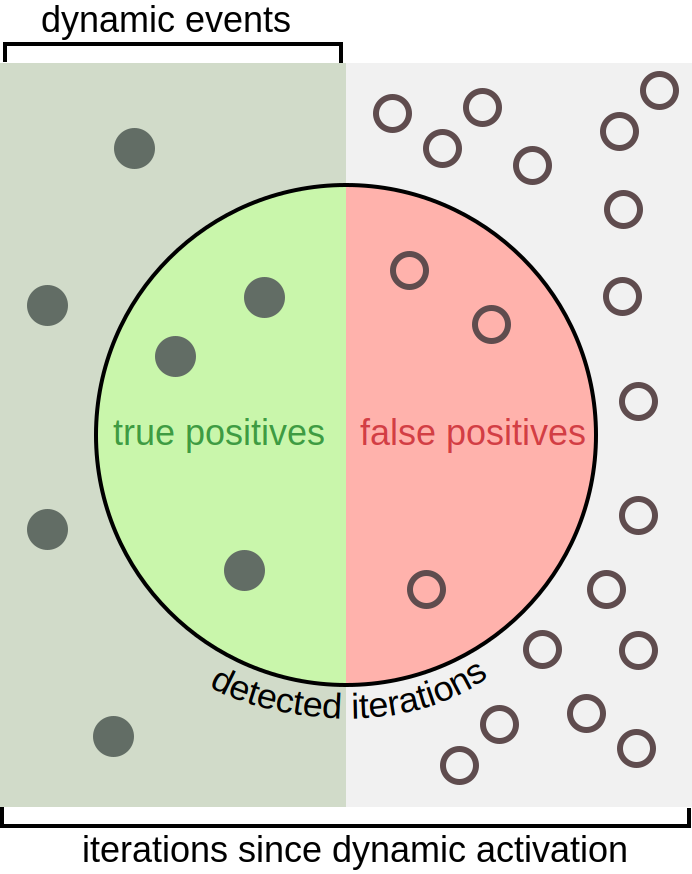
\includegraphics[width=0.45\textwidth]{dynamic_detection.svg}
	\caption[Illustration of iteration classification for dynamic problems]{Illustration of iteration classification for dynamic problems. Each dot represents one iteration between 2000 and 2600. The circle depicts all iterations where \gls{hsppbo} detected a dynamic change and therefore triggered the change handling procedure.}
	\label{fig:dynamic_detection}
\end{figure}